\section{Reduzierte Pendellänge}

Es soll vorbereitend die reduzierte Pendellänge berechnet werden, also die Länge, die ein mathematisches Pendel haben würde (eine punktförmiges Gewicht mit einem Faden mit vernachlässigbarer Masse), damit es mit gleicher Schwingungsdauer schwingen würde, wie das zu beschreibende physikalische Pendel. Das physikalische bzw. Reversionspendel Abb \ref{fig:Versuch 1.2}, für das die reduzierte Pendellänge berechnet werden soll, besteht aus einem zylindrischen, an einem Ende drehbar aufgehängte Stab der Länge L.

\begin{figure}
    \centering
    \includegraphics[scale=0.8]{Pendel/Protokoll/fig/Versuch 1.2.png}
    \caption{Physikalisches Pendel zur bestimmung der Fallbeschleunigung}
    \label{fig:Versuch 1.2}
\end{figure}

\begin{figure}[ht]
    \centering
    \includegraphics[scale=0.3]{Pendel/Protokoll/fig/Mathematisches Pendel.png}
    \caption{Mathematisches Pendel}
    \label{fig:Mathematisches Pendel}
    Quelle: Eichler Kronfeld Sahm "Das Neue Physikalische Grundpraktikum"
\end{figure}

\begin{figure}[ht]
    \centering
    \includegraphics[scale=0.3]{Pendel/Protokoll/fig/Physikalisches Pendel.png}
    \caption{Physikalisches Pendel}
    \label{fig:Physikalisches Pendel}
    Quelle: Eichler Kronfeld Sahm "Das Neue Physikalische Grundpraktikum"
\end{figure}

Nach der Grundgleichung für Drehbewegungen gilt:

\begin{equation} \label{Grundgleichung Drehbewegung}
    M = I \cdot \ddot{\varphi}
\end{equation}

wobei $M$ das rücktreibende Drehmoment, $I$ das Trägheitsmoment des Pendels und $varphi$ die Winkelbeschleunigung ist. Für das rücktreibende Drehmoment gilt: $M = -m \cdot g \cdot s \cdot \sin{\varphi}$ mit der Kleinwinkelnäherung $\sin{\varphi}$ folgt nach Einsetzen in Gleichung \ref{Grundgleichung Drehbewegung}:

\begin{equation} \label{Schwingungsgleichung eines physikalischen Pendels}
\ddot{\varphi} + \omega^2\varphi = 0
\Rightarrow \varphi = e^{i \omega t} \text{, mit } \omega = \sqrt{\frac{mgs}{I}}
\end{equation}

Mit dem Ergebnis für die Kreisfrequenz $\omega$ lässt sich nun die Persiodendauer $T$ berechnen:

\begin{equation}
    T = \frac{2\pi}{\omega} = 2 \pi \sqrt{\frac{I}{mgl}}
\end{equation}

Das Trägheitsmoment eines Zylinders mit einer homogenen Masseverteilung ist gegeben durch $I_Z = \frac{1}{3} ml^2$. Der Schwerpunkt des Zylinders liegt bei $s = l/2$. Daraus folgt für die Periodendauer des physikalischen Pendels:

\begin{equation}
    T = 2 \pi \sqrt{\frac{I}{mgs}} = 2 \pi \sqrt{\frac{\frac{1}{3} l^2}{mg\frac{l}{2}}} = 2 \pi \sqrt{\frac{2l}{3g}}
\end{equation}

Durch einen Vergleich mit der Periodendauer eines mathematische Pendels:

\begin{equation} \label{Periodendauer mathematisches Pendel}
   T_m = 2 \pi \sqrt{\frac{l_r}{g}} 
\end{equation} 

lässt sich erkennen, dass die reduzierte Pendellänge $l_r = \frac{2}{3}l$ beträgt.

Weiter soll vorbereitend gezeigt werden, dass eine zusätzlich angebrauchte Masse bei $l_r$  keine Veränderung der Periodendauer hervorruft. Also gilt für $I^\prime = m^\prime (\frac{2}{3}l)^2$ und für $s^\prime = \frac{2}{3}l$

\begin{equation}
    T^\prime = 2 \pi \sqrt{\frac{I + I^\prime}{mgs+m^\prime g s^\prime }} = 2\pi \sqrt{ \frac{ (\frac{m}{2} + \frac{2}{3} m^\prime) \frac{2}{3}l^2} { (\frac{m}{2} + \frac{2}{3}m^\prime)g l  }} \equiv T
\end{equation}

Mit dieser Erkenntnis lässt sich argumentieren, dass die Klauen, an denen das Pendel aufgehängt wird, eine zu vernachlässigende Änderung der Periodendauer mit sich bringen.

\section{Bestimmung der Fallbeschleunigung g mit Hilfe des Reversionspendels}

Aus Gleichung \ref{Periodendauer mathematisches Pendel} erhält man durch umformen eine Formel für die Fallbeschleunigung: 

\begin{equation} \label{Fallbeschleunigung mathematisches Pendel}
    g = l_r \frac{4 \pi^2}{T^2}
\end{equation}

wobei in diesem Versuchsteil $l_r$ experimentell bestimmt werden soll, um somit die Fallbeschleunigung experimentell zu bestimmen. Dabei ist die Periodendauer gleich um beiden Schneiden, wenn $d = l_r$ gilt, wobei $d$ der Abstand der beiden Schneiden ist. Für die Bestimmung von $l_r$ wird eine Messreihe für verschiedene Abstände $d$ der beiden Schneiden (Abb. \ref{fig:Pendel Versuch 1.1}), wie man an dem Plot erkennen kann, folgt die Periodendauer für die Aufhängung an der festen Schneide einer Geraden, während dies für die bewegliche Schneide nicht der Fall ist, deshalb werden für die lineare Regression nur Datenpunkte in der Nähe vom Schnittpunkt gewählt, wo der Verlauf näherungsweise linear ist. Die reduzierte Länge erhält man nun, indem man den Schnittpunkt der beiden angepassten Gerade berechnet:

\begin{align} 
    \nonumber y_{fest} &=  1.4383s + 0.252 \cdot \frac{s}{m} x\\
    \nonumber y_{beweglich} &= 2.2040s -0.953 \cdot \frac{s}{m} x
\end{align}

Gleichsetzen und auflösen nach x liefert nun:

    $$x=l_r \approx 0.6354m $$
    Einsetzen liefert nun für die Periodendauer:
    $$T = y_{fest}(l_r) = y_{beweglich}(l_r) = 1.598 s$$

Damit erhalten wir nach einsetzen in die Gleichung \ref{Fallbeschleunigung mathematisches Pendel}:

$$ g = l_r \frac{4 \pi}{T^2} \approx 9.823 $$

Der Literaturwert für die Fallbeschleunigung beträgt $g=9.81 \frac{m}{s^2}$, unsere Abweichung beträgt demnach nur ungefähr $0.1 \% $

\begin{figure}[ht]
    \centering
    \includegraphics[scale=0.8]{Pendel/Protokoll/fig/Pendel Versuch 1.2.pdf}
    \caption{Daten Versuch 1.2}
    \label{fig:Pendel Versuch 1.1}
\end{figure}

\begin{figure}[ht]
    \centering
    \includegraphics[scale=0.8]{Pendel/Protokoll/fig/Pendel Versuch 1.2 Fit.pdf}
    \caption{Fit Versuch 1.2}
    \label{fig:Pendel Versuch 1.1 Fit}
\end{figure}